\begin{figure}[h]
\begin{center}
	\begin{subfigure}{0.49\textwidth}
		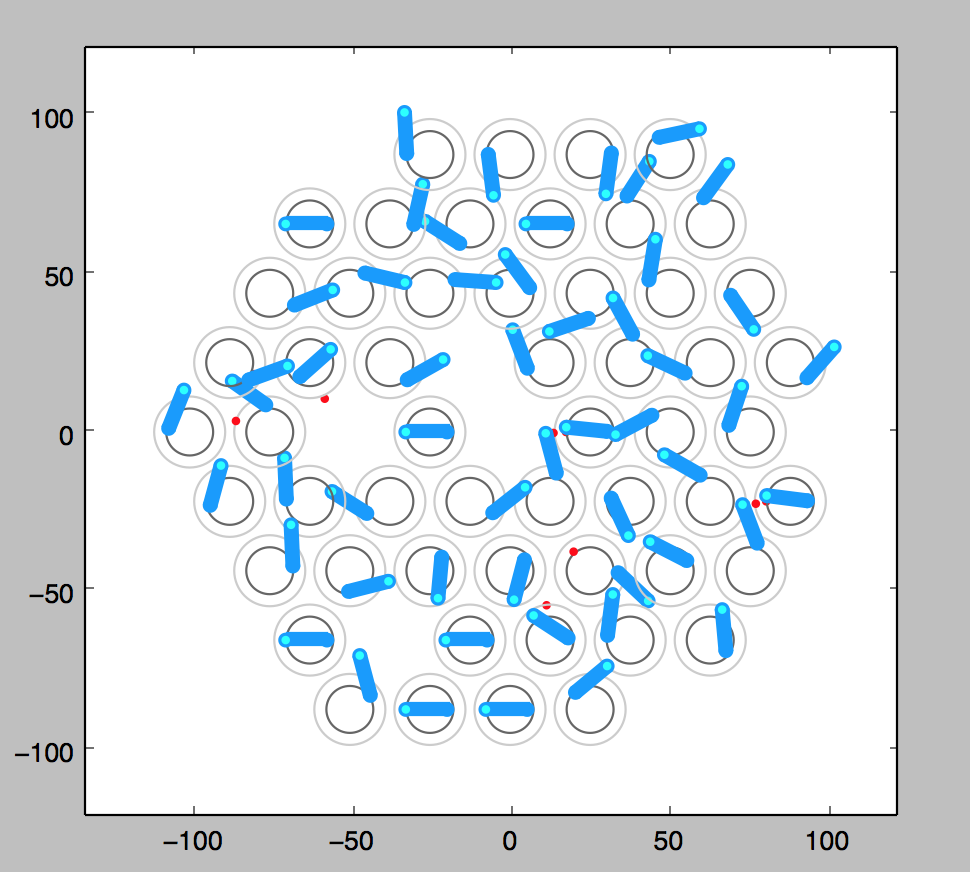
\includegraphics[width=0.9\textwidth]{set_target/sans_correction.png}
		\caption{Résultats pour 60 positionneurs, sans la correction.}
		\label{fig:correction:normal}
	\end{subfigure}
	\begin{subfigure}{0.49\textwidth}
		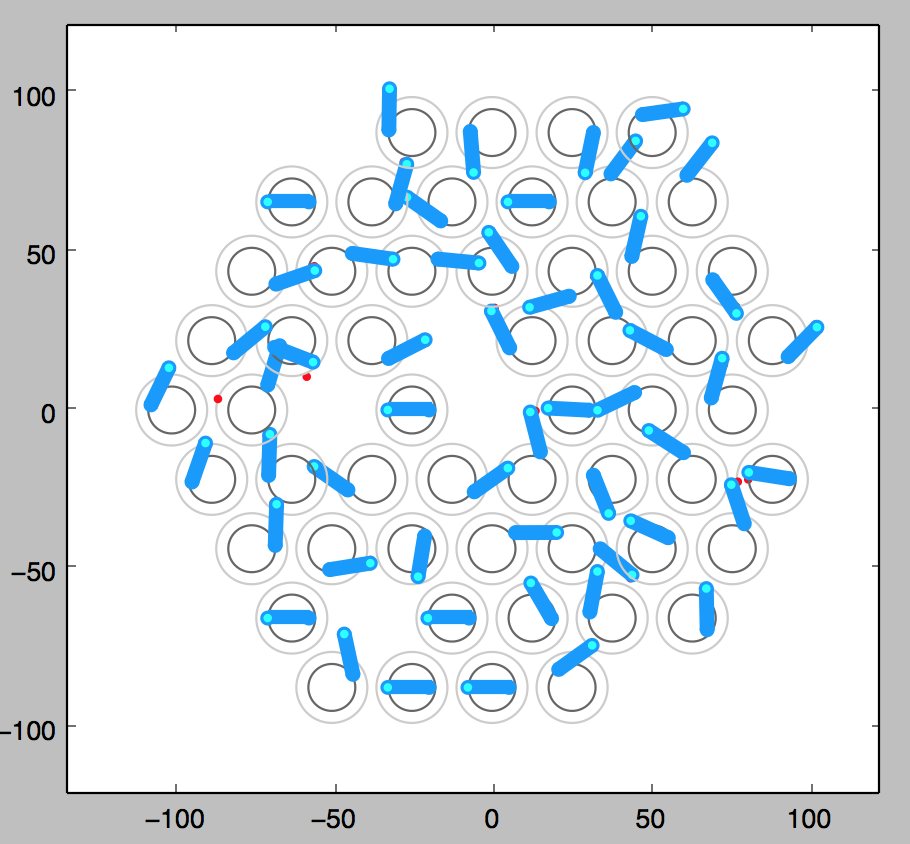
\includegraphics[width=0.9\textwidth]{set_target/correction.png}
		\caption{Résultats pour 60 positionneurs, avec la correction du système.}
		\label{fig:correction:normal}
	\end{subfigure}
	
	\begin{subfigure}{0.49\textwidth}
		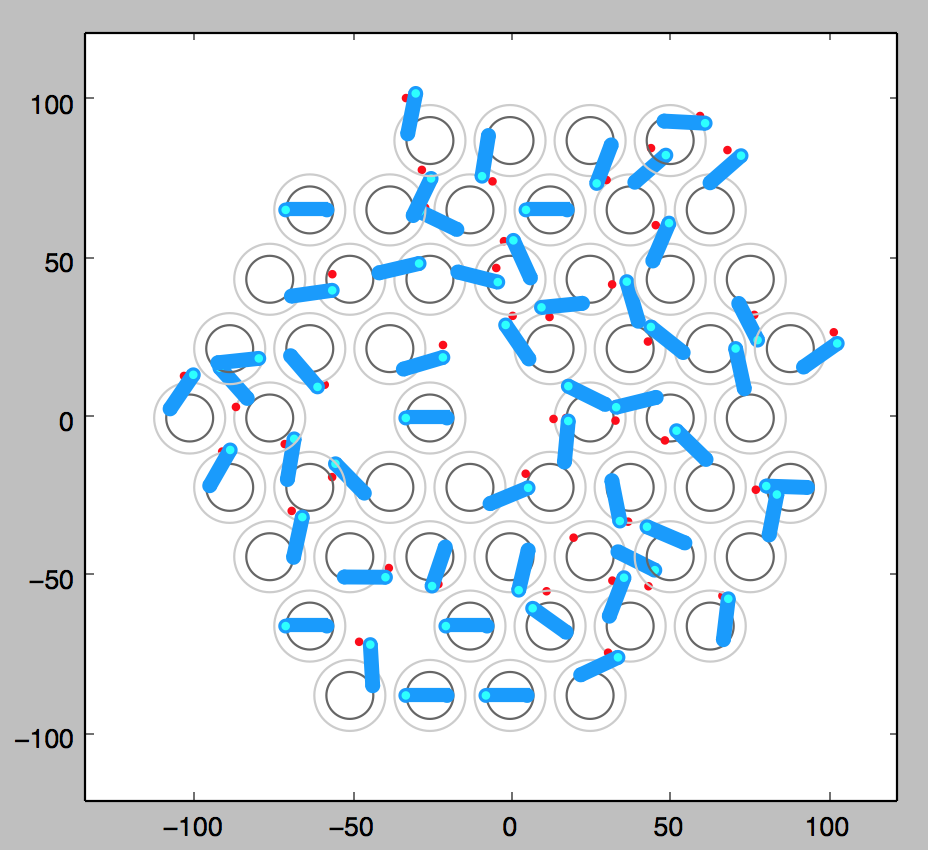
\includegraphics[width=0.9\textwidth]{set_target/correction_x4.png}
		\caption{Résultats pour 60 positionneurs, avec la correction du système multiplié par un facteur 4.}
		\label{fig:correction:normal}
	\end{subfigure}
	\begin{subfigure}{0.49\textwidth}
		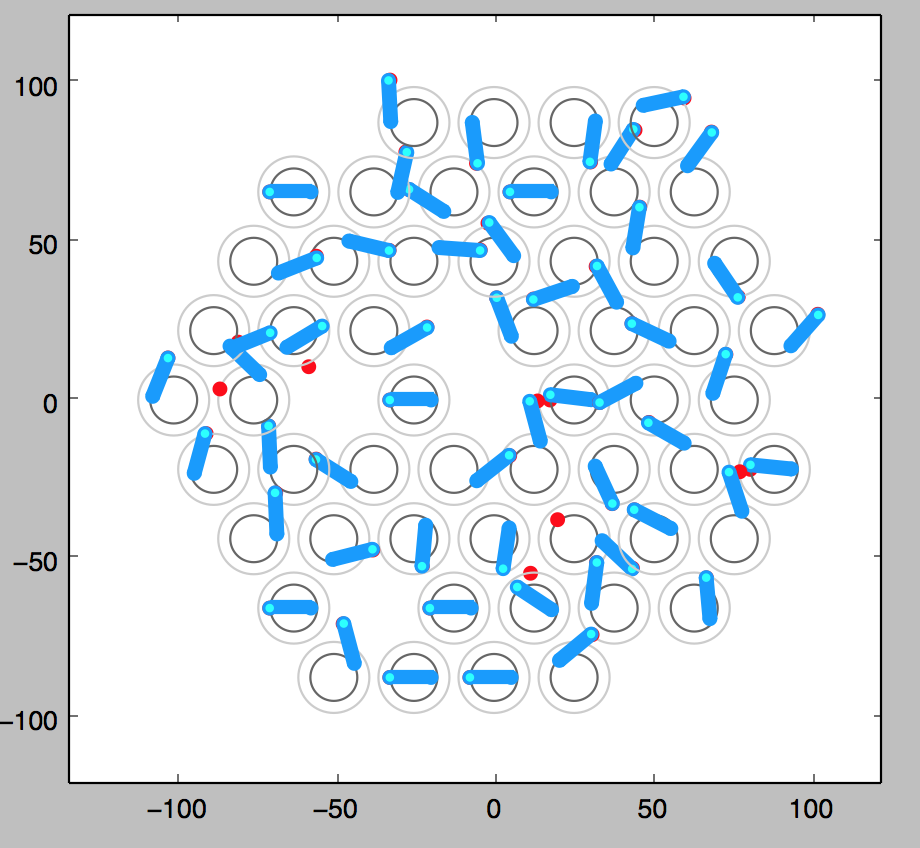
\includegraphics[width=0.9\textwidth]{set_target/sans_correction_r2.png}
		\caption{Résultats pour 60 positionneurs, sans la correction, en élargissant les rayons des targets d'un facteur 2.}
		\label{fig:correction:normal}
	\end{subfigure}
	
	\begin{subfigure}{0.49\textwidth}
		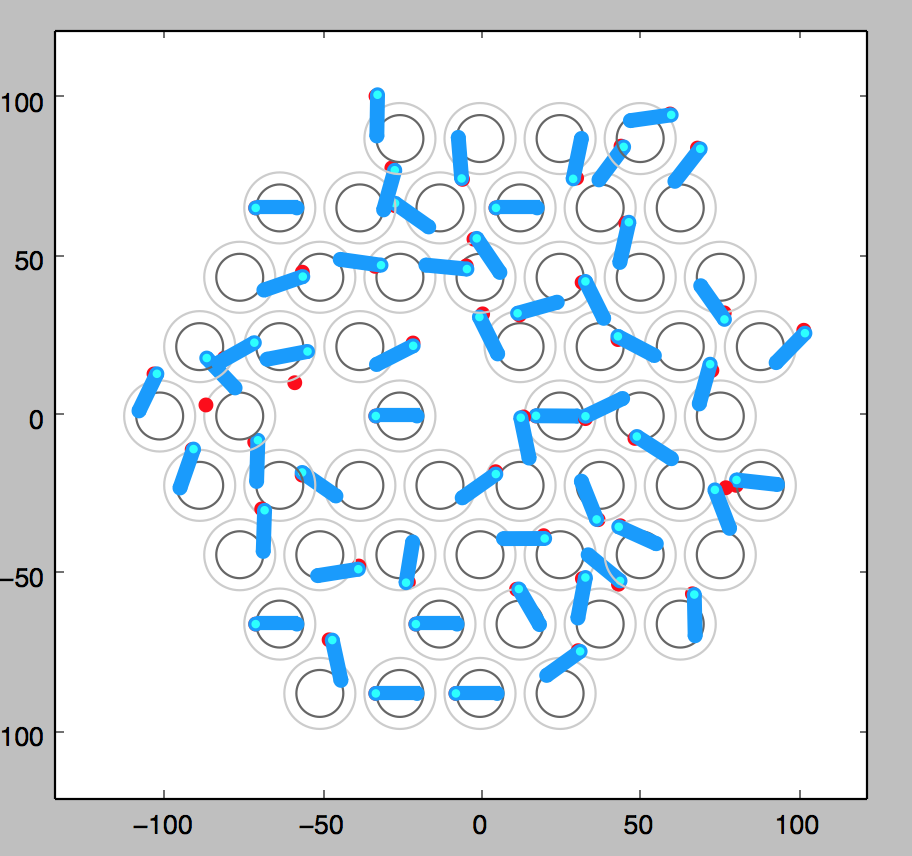
\includegraphics[width=0.9\textwidth]{set_target/correction_r2.png}
		\caption{Résultats pour 60 positionneurs, avec la correction du système, en élargissant les rayons des targets d'un facteur 2.}
		\label{fig:correction:normal}
	\end{subfigure}
	\begin{subfigure}{0.49\textwidth}
		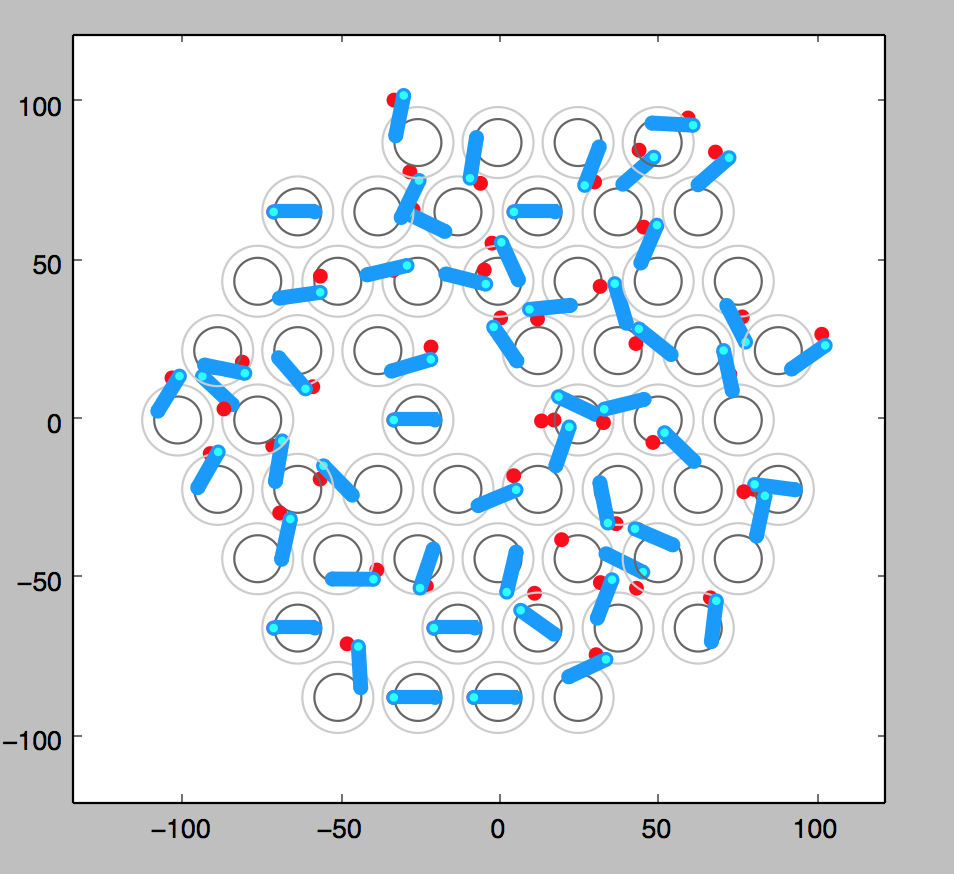
\includegraphics[width=0.9\textwidth]{set_target/correction_x4_r2.png}
		\caption{Résultats pour 60 positionneurs, avec la correction du système multiplié par un facteur 4, en élargissant les rayons des targets d'un facteur 2.}
		\label{fig:correction:normal}
	\end{subfigure}
\end{center}
\end{figure}